\documentclass{standalone}
\usepackage{PhysicalChemistryNote}
\begin{document}
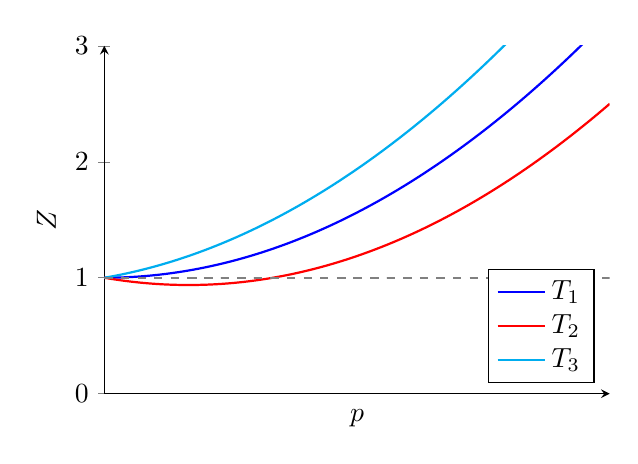
\begin{tikzpicture}
    \begin{axis}[
        width = 8cm,
        height = 6cm,
        legend pos = south east,
        xlabel = {$p$},
        ylabel = {$Z$},
        axis lines = left,
        ymin = 0,
        ymax = 3,
        xtick = \empty,
        domain = 0:3,
        samples = 400
    ]
    \addplot [thick, blue] {0.25*x^2+1};
    \addplot [thick, red] {0.25*(x-0.5)^2+15/16};
    \addplot [thick, cyan] {0.25*(x+0.5)^2+15/16};
    \addplot [thick, dashed, gray] {1};
    \legend {$T_1$,$T_2$,$T_3$}
    \end{axis}
\end{tikzpicture}
\end{document}